\section{Problem Descriptions}

\subsection{Question 1}
\subsubsection{Summary}
Interview Question 1 asks the interviewee to evaluate a short program.
The program passes a function as an argument, a concept the students might not be familiar with, but is a key concept of functional programming.
The program is 18 lines long and takes up less than a page when printed.
The problem can be found in the Appendix as Interview Question 1.
\subsubsection{Solution Description}

One (popular) way to determine the solution is to realize the only piece of code that gets executed at the top level is the call to main on line 18.
Then following the execution of the program, main prints out the result of \texttt{func3([1,2,3,4])}.
The functions func3 and func2 just add arguments, so the original call to main is equivalent to calling \texttt{func1([1,2,3,4],4,func4)}.
Note that func4 is being passed, thus when the parameter ``f'' is called in func1 on line 9 it is really calling the function func4.
Continuing the trace in func1, acc starts at $0$ then adds \texttt{func4(i,4)} for each ``i'' in the list.
Since func4 is just multiplication, this results in summing 4 times the elements of the list, which comes out to 40.
From there the program just repeatedly returns the 40, until it returns to main when we print 40.
This process can be seen in Figure \ref{fig-q1}.

\begin{figure*}[t]
\centering
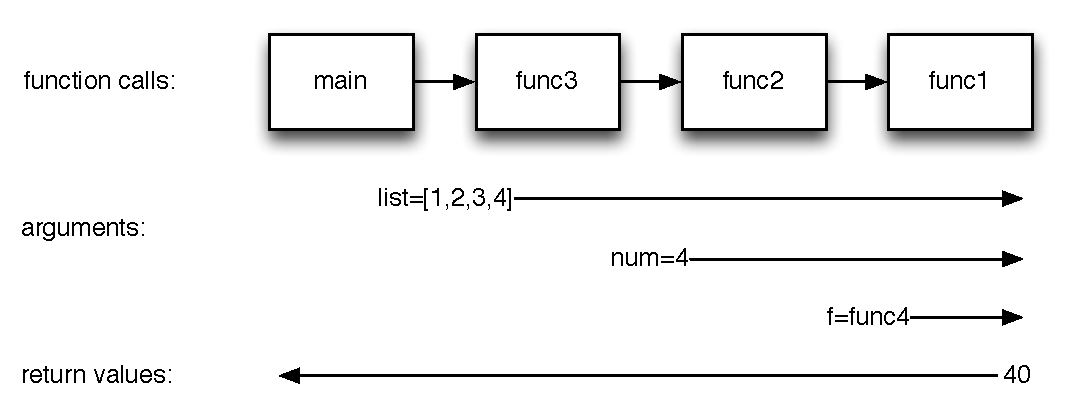
\includegraphics[width=1.0\textwidth]{Q1diagram.pdf}
\caption{Flow of Arguments and Return Values in Question 1}
\label{fig-q1}
\end{figure*}
 
%\newpage
\subsection{Q4}
\subsubsection{Summary}
Interview Question 4 (Q4) asks the interviewee to locate and fix a bug in a program that they are told plays Connect 4.
The bug is that when pieces are dropped into the board, the program lets pieces be dropped in even if the column is full.
The program is 70 lines long and covers two pages when printed.
The problem can be found in the Appendix as Interview Question 4.

\subsubsection{Solution Description}
\begin{figure*}[t]
\centering
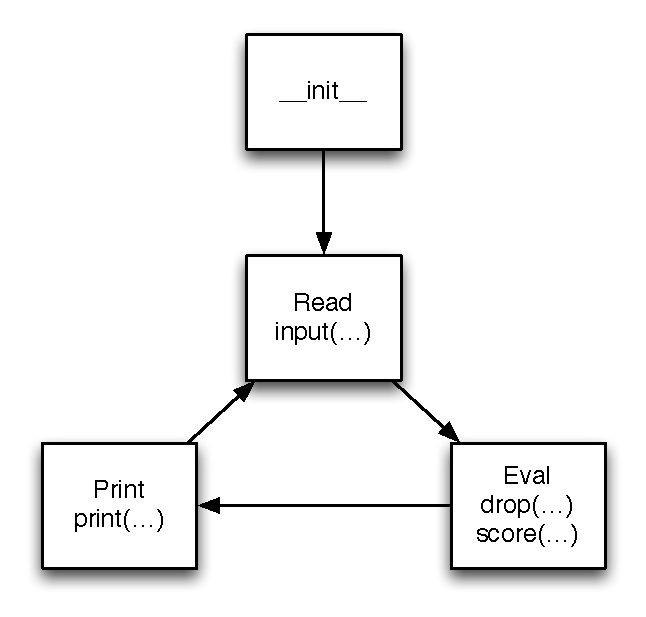
\includegraphics[width=0.5\textwidth]{Q4diagram.pdf}
\caption{Read-Eval-Print Loop and the important functions used in each part of the loop in Q4}
\label{fig-q2}
\end{figure*}

The following solution uses execution order to come to the correct conclusion. Other methods are possible. 

To find the correct solution we start at line 49 where the code starts executing.
Some variables are set up to be used later. 
Here a Board is initialized.
It calls the \_\_init\_\_ function (line 3) which creates a list of lists stored as the self.board variable.
The initial lists are empty.
It also stores the height and width of the board in class variables. \\

Here the program starts a Read-Eval-Print loop. A Read-Eval-Print loop is a structure that takes in input, evaluates how that changes the stored data, and then prints a representation of the data. Figure \ref{fig-q2} shows the structure of this loop and the previous initialization as well as the function calls that correspond to each part of the loop.\\

At line 55, the program asks for input, the read part of the loop.
Then, it calls the drop(player,c) function which adds a piece to the column that the user has specified through the input.
In the drop function (line 8), we can see that if the column selected is part of the self.board variable,
	the piece is appended to that column in the list of lists.
This is analogous to dropping a piece into the Connect 4 board in an actual game, meaning this is a logical place where the bug could be fixed.\\

Since we check that the column is valid,
we can also check that the column is not full by changing the drop function to include this line between lines 9 and 10:
if len(self.board[column]) $<$ self.height:.
This code will make sure that pieces will not be dropped in full columns.\\

Other possible solutions that cause the drop function to not be called if the column is full would also be acceptable.

\newpage
